\documentclass[a4paper,11pt]{uzreport}
\author{
  Erwin Konkel\\
  Mateusz Znojek\\
  Stanisław Mól - Scrum Master\\
}
\group{33INF-SSI-SP/B}
\class{Część teoretyczna}
\labnumber{Zaawansowane technologie usług sieciowych}
\date{19.01.2021}
\supervisor{dr inż. Piotr Powroźnik}

\begin{document}
  \maketitle
  
\section{Opis systemu}
	System przeznaczony do nakładania planu zajęć Uniwersytetu Zielonogórskiego na czytelną siatkę, na wzór do kalendarza google. Użytkownik ma możliwość wyboru kierunku, grupy oraz podgrupy, względem której ma zostać zmapowany plan. Informacje te zostaną zapamiętane dla zalogowanego użytkownika.
    
    \begin{itemize}[leftmargin=0.50in]

        \item Grupą docelową systemu są studenci Uniwersytetu Zielonogórskiego.

	\item Grupą opcjonalną, która mogła by w przyszłości korzystać z możliwości planu, są osoby prowadzące zajęcia.

    \end{itemize}

\section{Opis istniejących rozwiązań}
	Najszerzej znanym rozwiązaniem jest "G Suit" działający w chmurze obliczeniowej pakiet zwiększający produktywność oraz oprogramowanie do pracy grupowej i oprogramowanie oferowane przez Google na zasadzie subskrypcji. Na jego podstawie można wywnioskować, że czytelność planu odgrywa główną rolę i właśnie na tym aspekcie zostanie skupiony porojekt. Głównym elementem na którym wzorowany będzie cały projekt jest kalendarz google widocznym na rysunku \ref{kalendarz_google_1}.\\

    \begin{figure}[ht!]
        \centering
        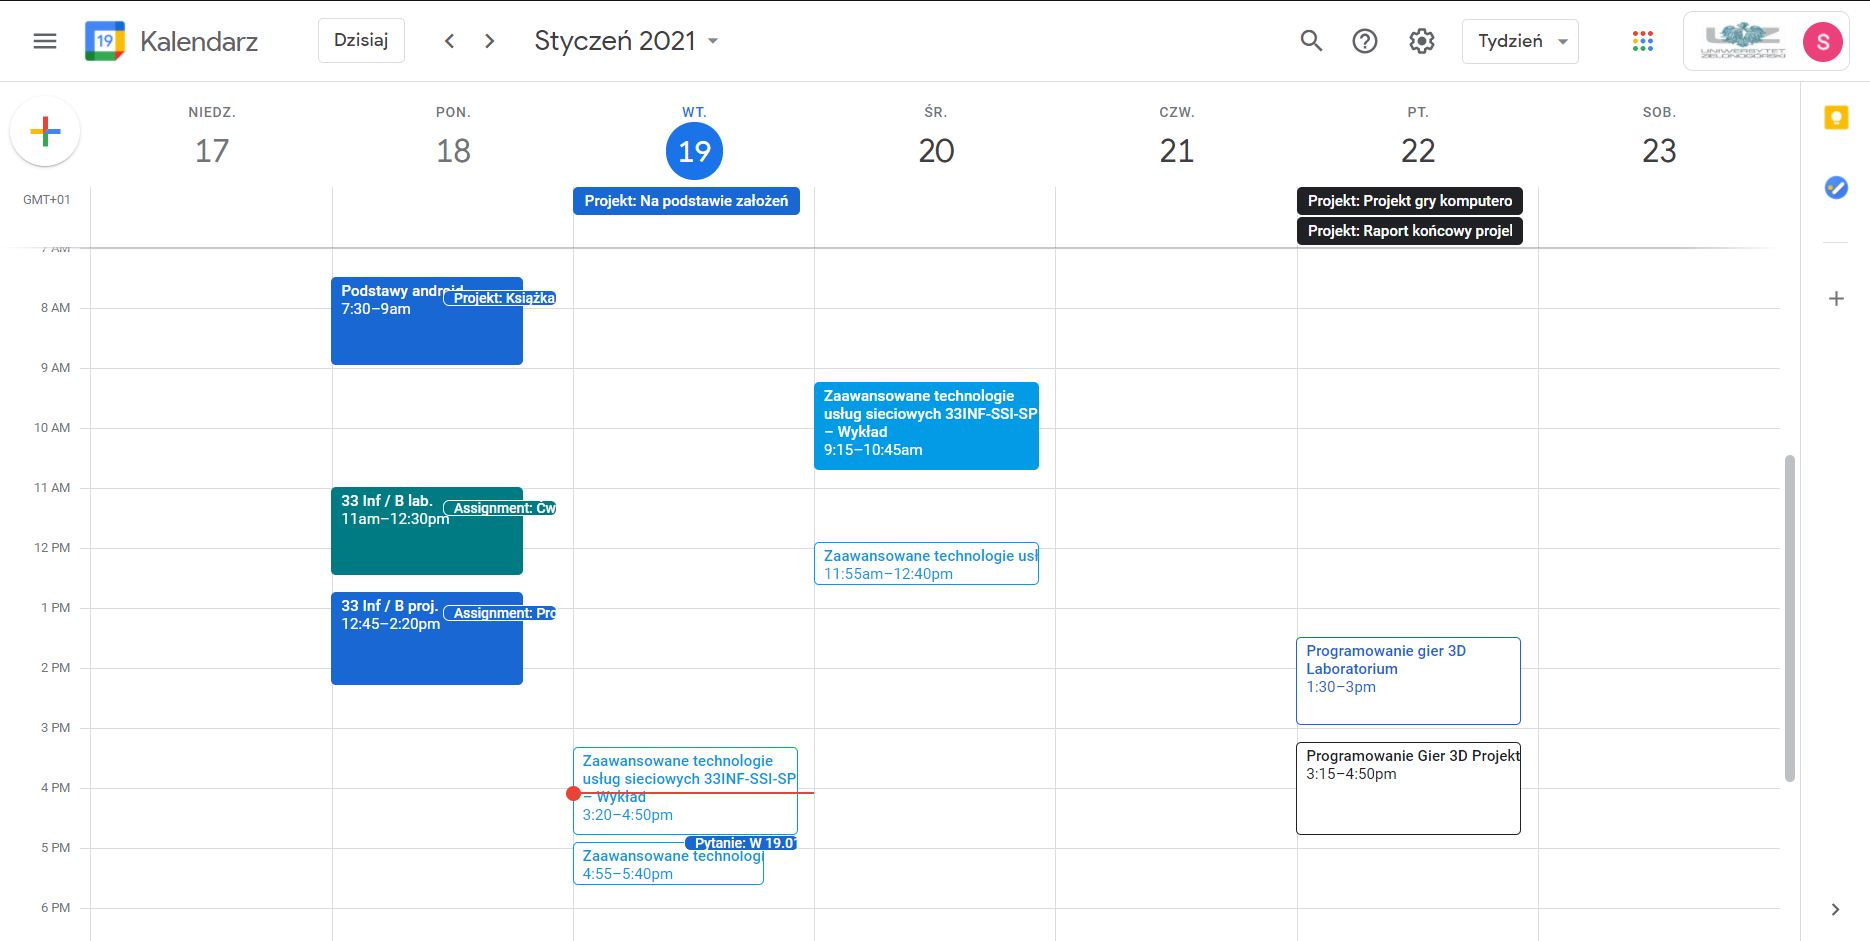
\includegraphics[width=0.9\textwidth]{pictures/Kalendarz-Google_1.jpg}
        \caption{Kalendarz Google}
        \label{kalendarz_google_1}
     \end{figure}

\clearpage
\section{Funkcjonalności}

\begin{center}
\begin{tabular}{ |m{8cm} | m{8cm} | } 
\hline
\textbf{Niezalogowany użytkownik} 									& \textbf{Zalogowany użytkownik}						\\
\hline
logowanie	 													&wylogowanie										\\ 
\hline
rejestracja														&możliwość dodania własnego zdarzenia					\\ 
\hline
wybór grupy dziekańskiej bez możliwości zapamiętania wyboru				&wybór grupy dziekańskiej z możliwością zapamiętania wyboru	\\ 
\hline
podgląd planu zajęć wybranej grupy dziekańskiej							&podgląd swojego planu								\\ 
\hline
wybór motywu													&możliwość dodania informacji o kolokwium do zajęć			\\ 
\hline
-															&wysłanie powiadomienia e-mail z przypomnieniem			\\ 
\hline
-															&wyszukiwanie wykładowcy							\\ 
\hline
-															&wybór motywu										\\ 
\hline
-															&edycja zdarzeń zawartych w kalendarzu					\\ 
\hline
-															& tablica TODO										\\ 
\hline
\end{tabular}
\end{center}
    
\section{Opis funkcjonalności}
    
    \begin{itemize}[leftmargin=0.50in]
    
        \item \textbf{Rejestracja / Logowanie / Wylogowanie} - prosta funkcjonalność pozwalająca na zarejestrowanie się użytkownika, następnie autoryzację na 			podstawie podanego loginu i hasła, oraz wylogowanie po zakończonej sesji.
        
        \item \textbf{Wybór grupy dziekańskiej} - użytkownik niezalogowany będzie miał możliwość wyboru grupy i podglądu planu zajęć dla danej grupy, jednakże 			nie będzie miał możliwości zapamiętania tego wyboru. Dla użytkownika zalogowanego będzie istniała możliwość zapamiętania wybranej grupy, początkowo 			wybór ten będzie możliwy podczas rejestracji, lecz będzie można zmienić wybór w panelu użytkownika.
        
        \item \textbf{Podgląd planu} - plan będzie wyświetlany w czytelnej formie, dzięki nałożeniu na siatkę czasu (podobnie jak w kalendarzu google).
        
        \item \textbf{Dodanie informacji o kolokwium do zajęć} - zalogowany użytkownik będzie miał możliwość dodania informacji czy na danych zajęciach 				zaplanowane jest kolokwium.
        
        \item \textbf{Dodanie własnego zdarzenia} - zalogowany użytkownik ma możliwość dodania własnego zdarzenia.
        
        \item \textbf{Wysłanie powiadomienia e-mail} - po wcześniejszym zaznaczeniu opcji system będzie wysyłał powiadomienie e-mail o zbliżających się 				kolokwiach (jeżeli są dodane).
        
        \item \textbf{Wyszukanie wykładowcy} - możliwość wyszukania wykładowcy w systemie i znalezienia potrzebnych informacji o wykładowcy.
        
        \item \textbf{Wybór motywu} - użytkownik może wybrać motyw aplikacji (ciemny / jasny).
        
        \item \textbf{Edycja zdarzeń} - użytkownik zalogowany ma możliwość edytowania zdarzeń na własnym planie.
        
        \item \textbf{Tablica TODO} - tablica z zadaniami do wykonania na następny dzień.
        
    \end{itemize}

\section{Opis problemów}
	Główne problemy przewidziane podczas projektowania, oraz proponowane rozwiązania:

	\begin{itemize}[leftmargin=0.5in]

		\item Stworzenie bazy danych - ważne zaganienie które może być problematyczne - rozwiązaniem problemu może być użycie 'Hibernate'.
            
		\item Przechowywanie danych użytkowników w bazie - jednym z problemów będzie przechowywanie danych wrażliwych takich jak hasła - 			 			rozwiązaniem tego problemu będzie przechowywanie zahashowanych danych.
                
 	\end{itemize}

\section{Diagram bazy danych i relacji}

	Diagram bazy danych prezentuje się jak na rysunku \ref{diagram_bazy_danych}. Trzonem łączącym grupy jest grupa, która posiada najważniejsze relacje łączące studenta z danymi o konkretnych zajęciach.

    \begin{figure}[ht!]
        \centering
        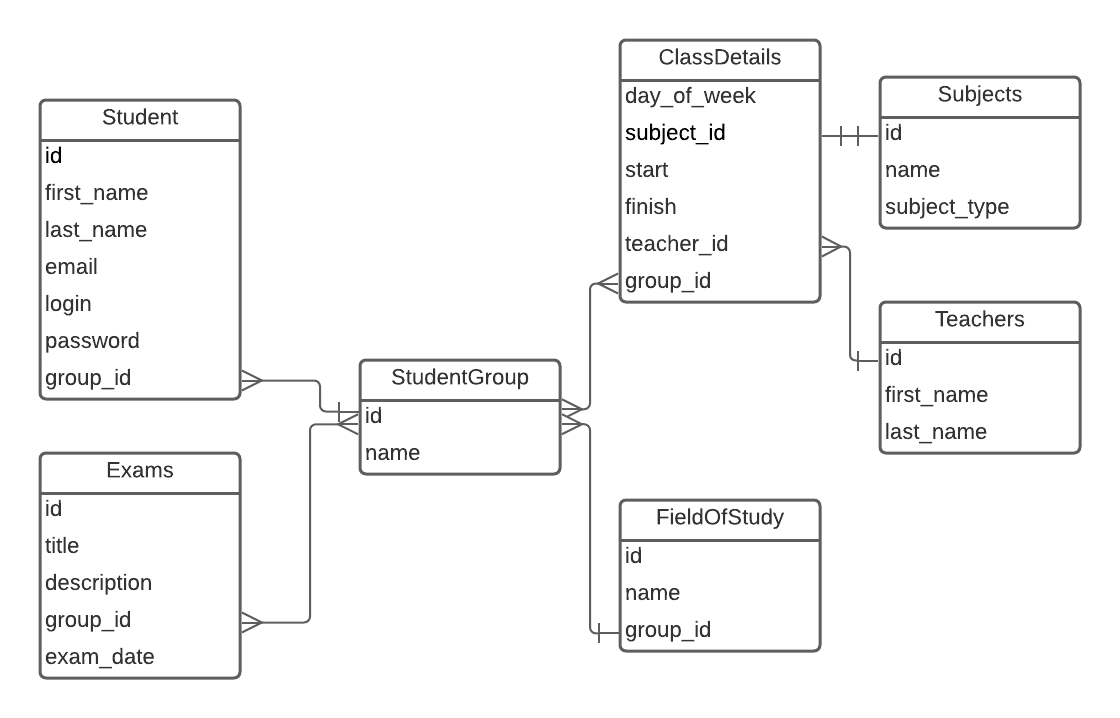
\includegraphics[width=0.9\textwidth]{pictures/UZplaner-baza-danych.png}
        \caption{Diagram bazy danych}
        \label{diagram_bazy_danych}
     \end{figure}

\section{Diagram użycia}

    Diagram użycia prezentuje sie jak na rysunku \ref{diagram_uzyca}. Prezentuje on podstawowe funkcjonalności na których się skupiliśmy w budowie tej platformy tj. wyświetlanie odpowiednio sformatowanej tabeli z zajęciami konkretnej grupy lub zarejestrowanego użytkownika.

    \begin{figure}[ht!]
        \centering
        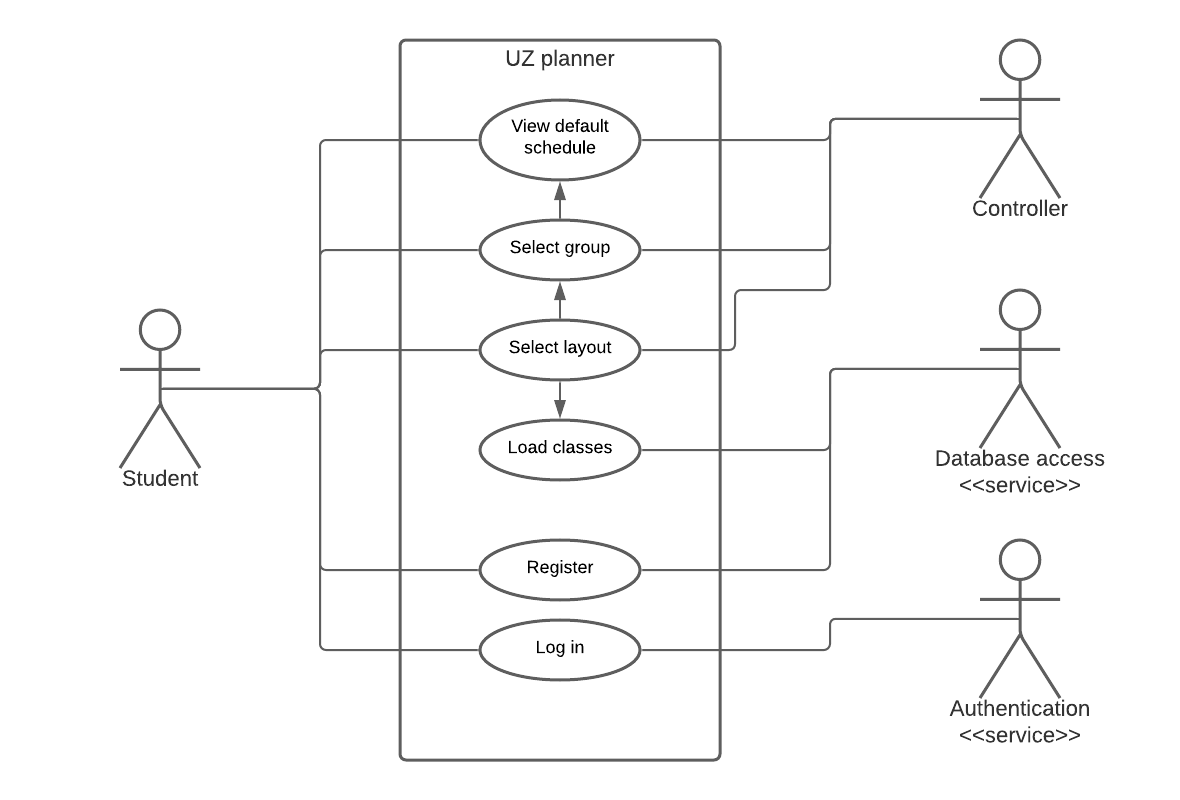
\includegraphics[width=0.9\textwidth]{pictures/use_case.png}
        \caption{Diagram użycia (\textit{Use Case})}
        \label{diagram_uzyca}
     \end{figure}

\section{Tabele przypadków użycia}

    Tabele przypadków użycia to kolejno dla każdej funkcjonalności: rejestracja rysunek \ref{fig4}, logowanie rysunek \ref{fig5}, zmiana motywu platformy \ref{fig6}, wyświetlanie głównego widoku planu rysunek \ref{fig7}, wybieranie grupy rysunek \ref{fig8}, wybieranie układu widoku planu rysunek \ref{fig9} \\

    \begin{figure}[ht!]
        \centering
        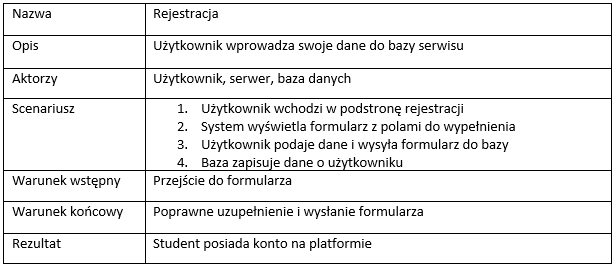
\includegraphics[width=0.9\textwidth]{pictures/rejestracja.PNG}
        \caption{Tabela rejestracji}
        \label{fig4}
     \end{figure}

     \begin{figure}[ht!]
        \centering
        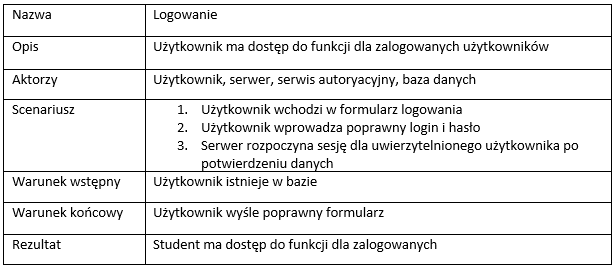
\includegraphics[width=0.9\textwidth]{pictures/logowanie.PNG}
        \caption{Tabela logowania}
        \label{fig5}
     \end{figure}

     \begin{figure}[ht!]
        \centering
        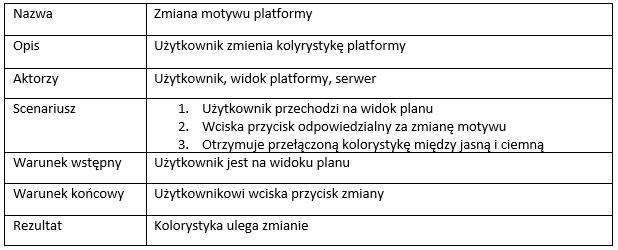
\includegraphics[width=0.9\textwidth]{pictures/zmiana_motywu.PNG}
        \caption{Tabela zmiany motywu}
        \label{fig6}
     \end{figure}

     \begin{figure}[ht!]
        \centering
        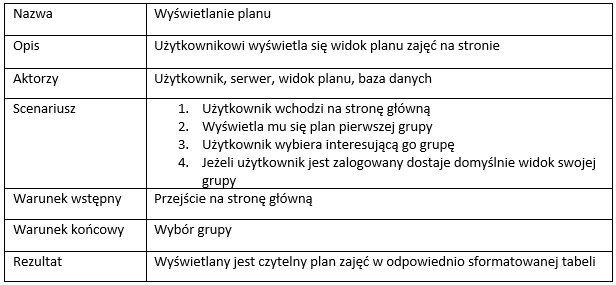
\includegraphics[width=0.9\textwidth]{pictures/wyswietlanie planu.PNG}
        \caption{Tabela wyświetlania planu}
        \label{fig7}
     \end{figure}

     \begin{figure}[ht!]
        \centering
        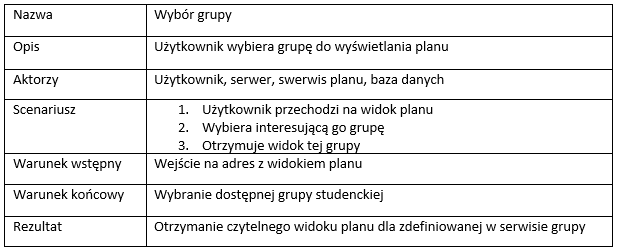
\includegraphics[width=0.9\textwidth]{pictures/wybor grupy.PNG}
        \caption{Tabela wyboru grupy}
        \label{fig8}
     \end{figure}

     \begin{figure}[ht!]
        \centering
        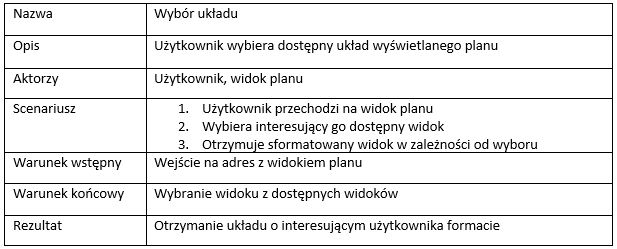
\includegraphics[width=0.9\textwidth]{pictures/wybor ukladu.PNG}
        \caption{Tabela wyboru układu}
        \label{fig9}
     \end{figure}

\clearpage
\section{Diagram komponentów/obiektów}

	\begin{figure}[ht!]
        	\centering
        	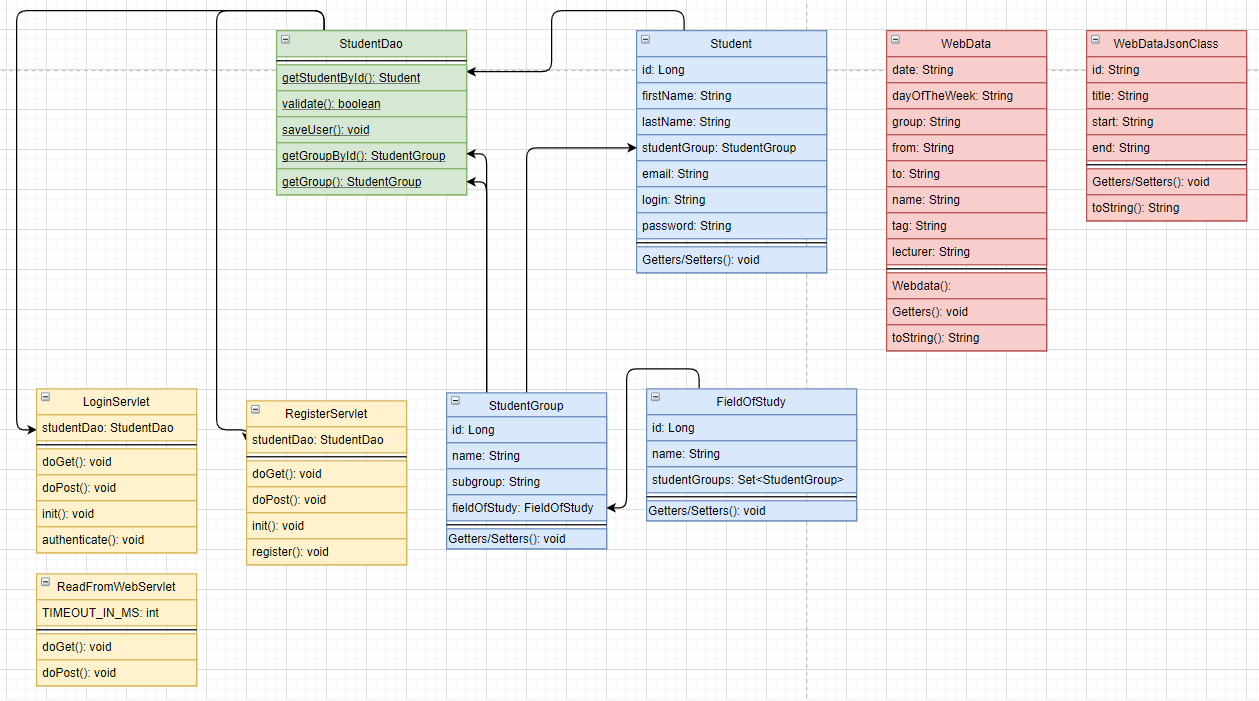
\includegraphics[width=0.8\textwidth]{pictures/Diagram_klas.png}
        	\caption{Diagram klas}
       		\label{diagram_klas}
     	\end{figure}

\section{Diagram przepływu sterowania}
	\begin{figure}[ht!]
        	\centering
        	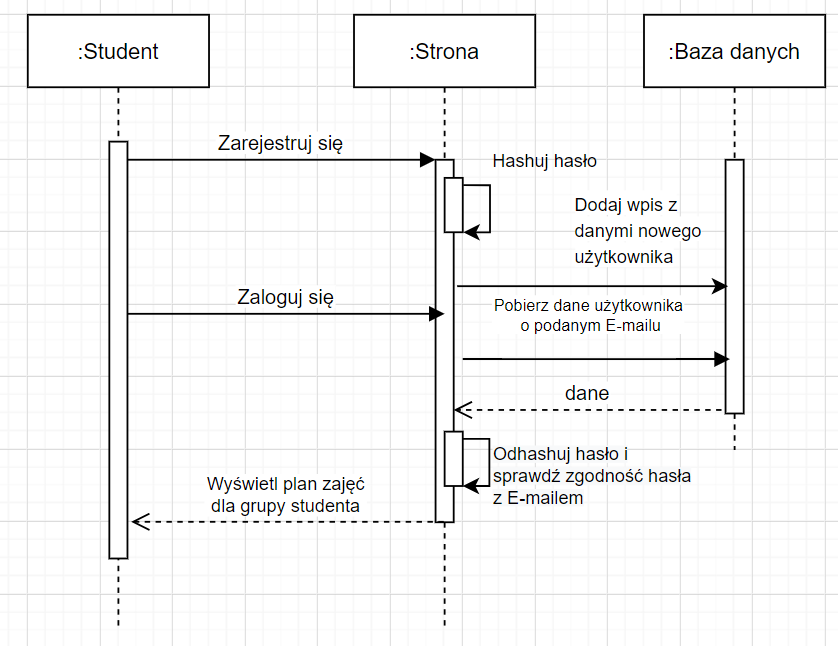
\includegraphics[width=0.8\textwidth]{pictures/diagram.png}
        	\caption{Diagram przepływu sterowania}
       		\label{diagram_przeplywu_sterowania}
     	\end{figure}

\section{Diagram funkcjonalny/strukturalny}
    Diagram strukturalny prezentuje sie jaka na rysunku \ref{diagram_funkcjonalny}. Platforma po otwarciu ładuje postawowe struktury danych czyli klasę odpowiedzialną za parsowanie wszystkich zajęć i wysyłanie ich do reszty komponentów oraz jednocześnie klasa pomocnicza która konwertuje dane na format json. Następnie ładowany jest główny widok planu wraz z jego komponentami w formacie jsp. Dalej ładowane są grupy oraz kierunki które można wybrać z bazy danych. Wybrana grupa wysyłana jest do serwisu odpowiedzialnego za dane do wyświetlenia i zapytanie zostaje obsłużone oraz zwracane są odpowiednie zajęcia. W przypadku zalogowanego użytkownika jego grupa ładowana jest automatycznie
    \begin{figure}[ht!]
        \centering
        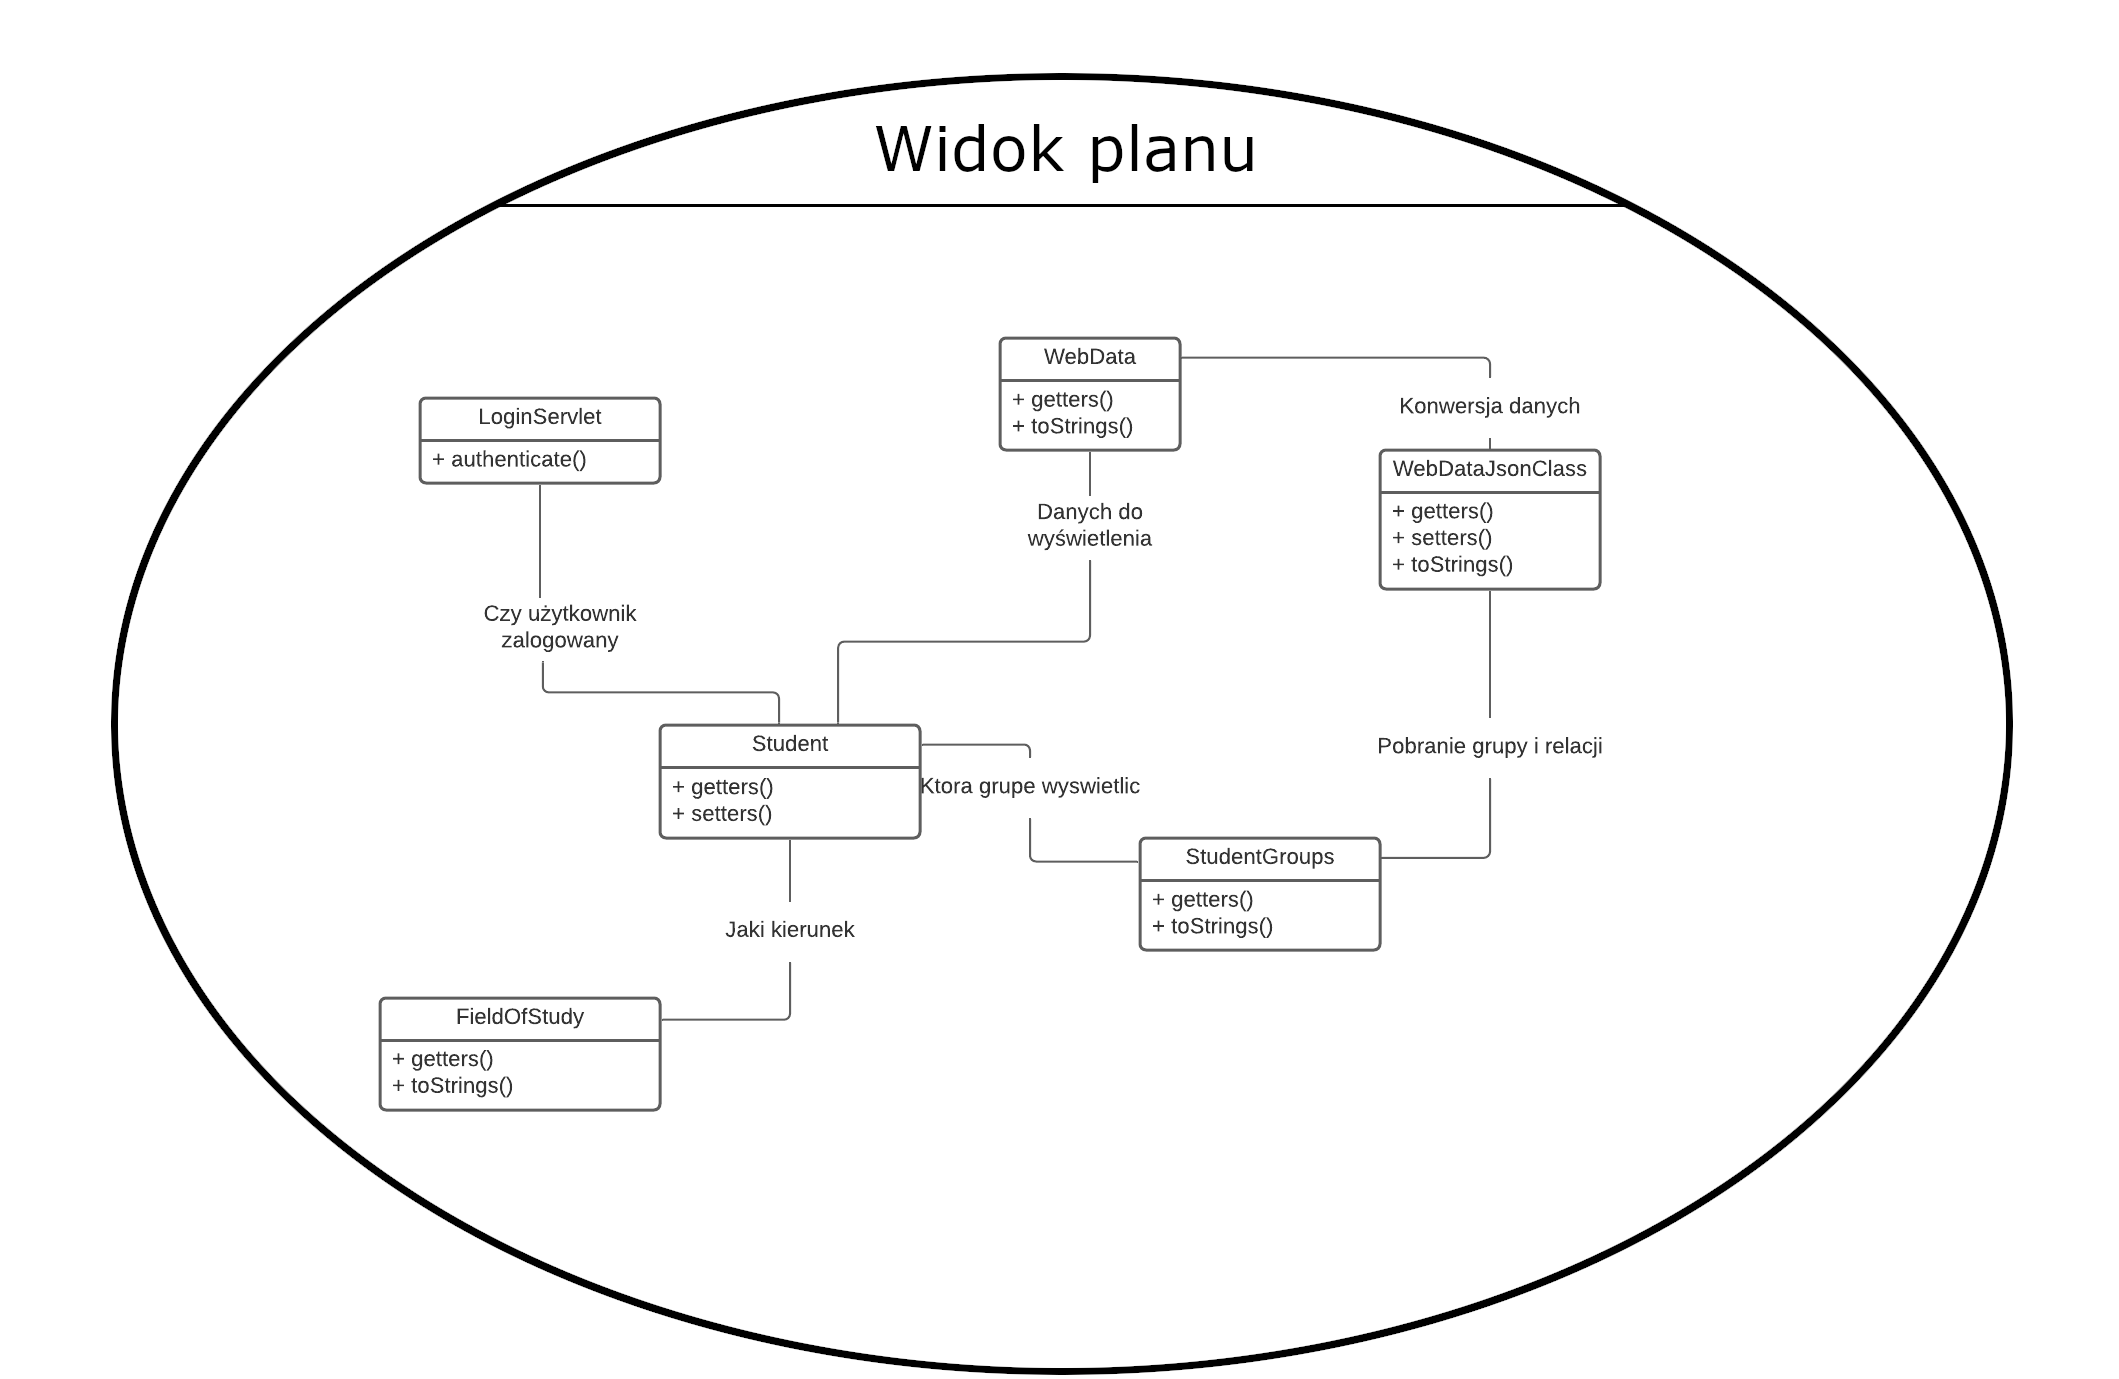
\includegraphics[width=0.9\textwidth]{pictures/Diagram_funkcjonalny.png}
        \caption{Diagram strukturalny}
        \label{diagram_funkcjonalny}
     \end{figure}

\clearpage
\section{MOSCOW}

\begin{center}
\begin{tabular}{ |m{4cm} | m{4cm} |m{4cm} | m{4cm} | } 
\hline
\textbf{Must} & \textbf{Should} & \textbf{Could} & \textbf{Won’t Have}\\
\hline
logowanie 	& możliwość dodania własnego zdarzenia & możliwość dodania informacji o kolokwium do zajęć & wybór motywu\\ 
\hline
wybór grupy dziekańskiej bez możliwości zapamiętania wyboru	& wysłanie powiadomienia e-mail z przypomnieniem & - & wyszukiwanie wykładowcy\\ 
\hline
podgląd planu zajęć wybranej grupy dziekańskiej 				& edycja zdarzeń zawartych w kalendarzu & - & tablica TODO\\ 
\hline
wylogowanie 										& - & - & -\\ 
\hline
rejestracja	& - & - & -\\ 
\hline
wybór grupy dziekańskiej z możliwością zapamiętania wyboru	& - & - & -\\ 
\hline
podgląd swojego planu 								& - & - & -\\ 
\hline
\end{tabular}
\end{center}

\section{Harmonogram zadań}
    
    \begin{figure}[ht!]
	\vspace{-15pt}
        \centering
        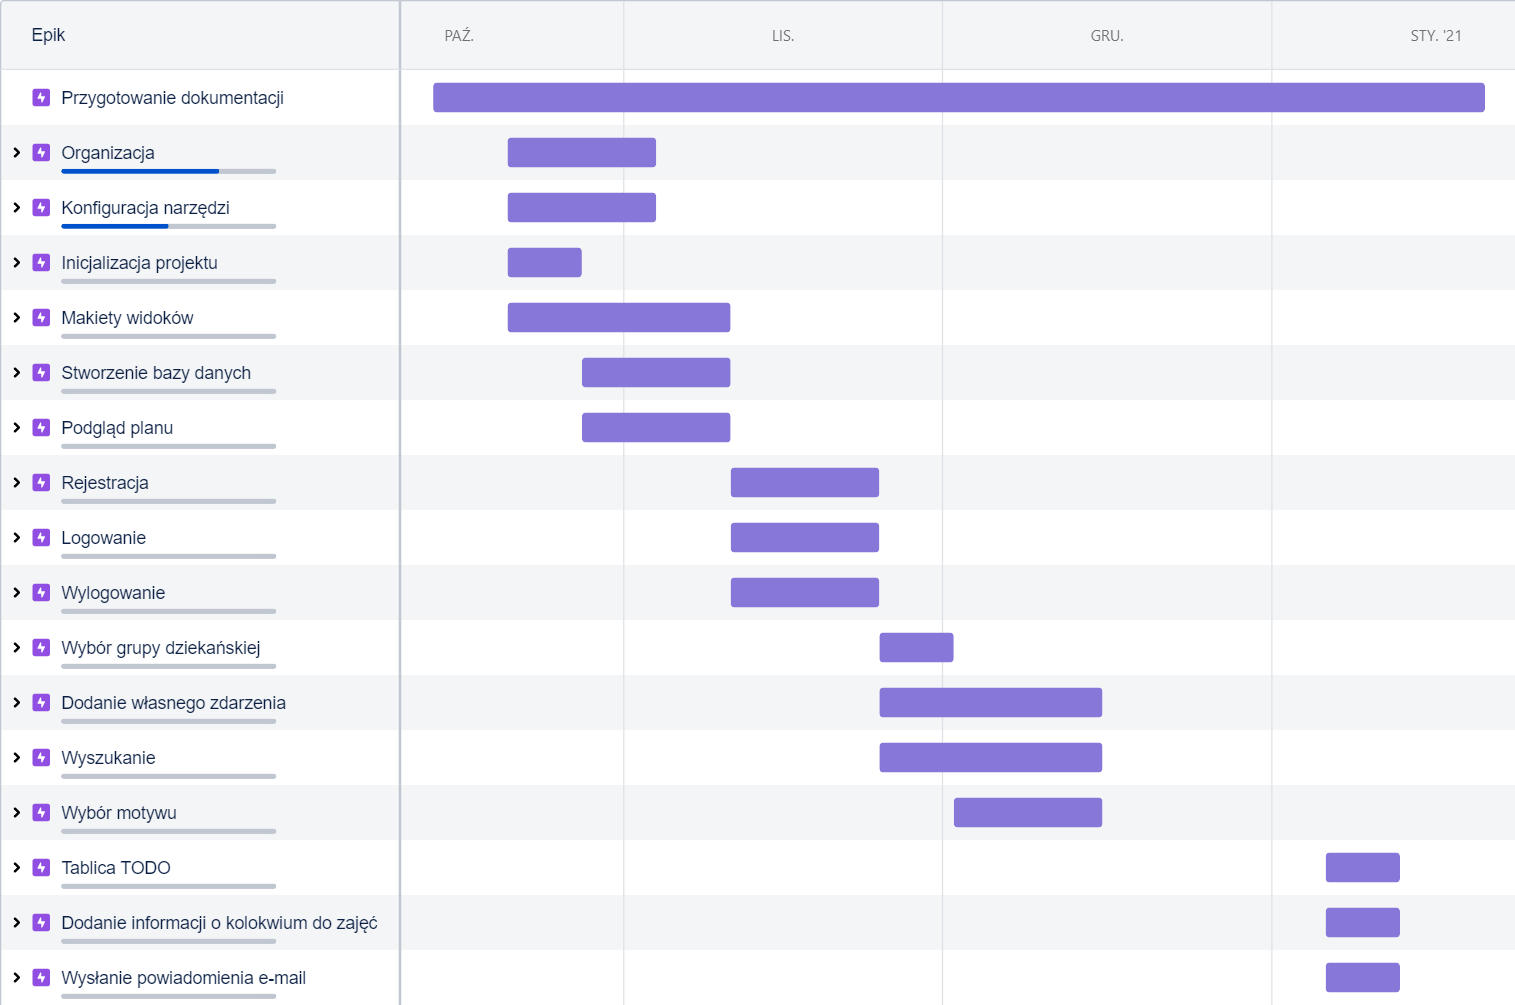
\includegraphics[width=0.9\textwidth]{pictures/fabulous_uz_planner_2020-10-27_06.13pm.png}
        \caption{Diagram Gantta}
	\vspace{-30pt}
     \end{figure}

\begin{center}
\begin{tabular}{ |m{6cm} | m{3cm}| m{3.5cm} | m{3cm} | } 
\hline
\textbf{Zadanie} 					& \textbf{Stanisław Mól} 	& \textbf{Mateusz Znojek} 		& \textbf{Erwin Konkel} \\ 
\hline
Przygotowanie dokumentacji 			& \checkmark			& 						&  \\ 
\hline
Organizacja 						& \checkmark 			& \checkmark 				& \checkmark \\ 
\hline
Konfiguracja narzędzi 					& \checkmark 			& \checkmark 				& \checkmark \\ 	
\hline
Inicjalizacja projektu					& \checkmark 			&  		 				&   \\ 
\hline
Makiety widoków					& 					&  		 				& \checkmark \\ 
\hline
Stworzenie bazy danych 				& 					& \checkmark 				&   \\ 
\hline
Podgląd planu 						& \checkmark 			&  		 				&   \\ 
\hline
Rejestracja 						& 					& \checkmark 				&   \\ 		
\hline
Logowanie 						& 					&  		 				& \checkmark \\ 
\hline
Wylogowanie 						&  					& \checkmark 				&   \\ 
\hline
Wybór grupy dziekańskiej 				&  					&  		 				& \checkmark \\ 
\hline
Dodanie własnego zdarzenia 			&  					& \checkmark 				&   \\ 
\hline
Wyszukiwanie 						& \checkmark 			&  		 				&   \\ 
\hline
Wybór motywu 						& 					& 		 				& \checkmark \\ 
\hline
Tabica TODO 						&  					& \checkmark 				&   \\ 
\hline
Dodanie informacji o kolokwium do zajęć 	& \checkmark 			& 		 				& \checkmark \\ 
\hline
Wysłanie powiadomienia e-mail 			& \checkmark			& \checkmark				& \checkmark \\ 
\hline
\end{tabular}
\end{center}

\section{Plan testów}

	Plan testów zakłada testowanie każdej historyjki przed oddaniem jej. Oznacza to, że każda funkcjonalność powinna zostać przetestowana przed dodaniem jej do głównej gałęzu projektu. Testy powinny być przeprowadzone na podstawie wyznaczonych kryteriów akceptacji.

\section{Plan bezpieczeństwa}

	Plan bezpieczeństwa zakłada dostarczenie możliwie uniwersalnych mechanizmów dla:
            \begin{itemize}[leftmargin=0.5in]
                \item uwierzytelniania (ang. authentication) - jestem tym za kogo się podaję bo: znam pin, znam hasło, mam takie odciski palców, posiadam certyfikat 			SSL, itp.
                \item autoryzacji (ang. authorization) - mam dostęp do określonych zasobów, a do innych nie
            \end{itemize}

    \begin{figure}[ht!]
        \centering
        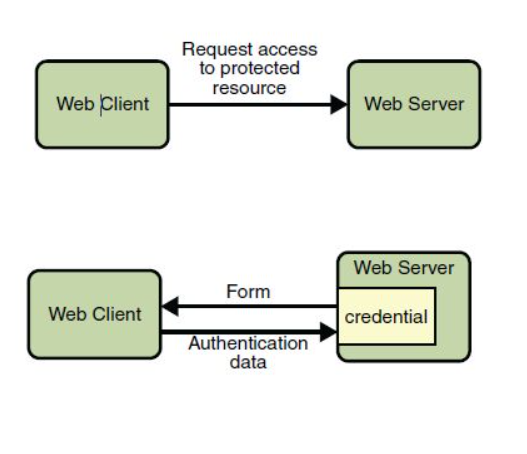
\includegraphics[width=0.8\textwidth]{pictures/uwierzytelnianie_klienta_web.png}
        \caption{Uwierzytelnienie klienta web}
        \label{fig10}
     \end{figure}

\section{Plan konserwacji}
Plan konserwacji obejmuje weryfikację oraz poprawanie błędów w trakcie implementacji każdej z nowych funkcjonalności, co oznacza, że każda funkcjonalność powinna zostać szczegółowo sprawdzona, po czym każdy z wykrytych błędów powinien zostać naprawiony. Po zakończeniu projektu, nie sa planowane kolejne aktualizacje.

\section{System kontroli wersji}
W projekcie został wykorzystany system kontroli wersji GIT ze względu na: 
	\begin{enumerate}[leftmargin=0.80in]
        	\item Dobre wsparcie dla rozgałęzionego procesu tworzenia oprogramowania
	       	\item Praca off-line: każdy programista posiada własną kopię repozytorium, do której może zapisywać zmiany bez połączenia z siecią      
        	\item Efektywna praca z dużymi projektami.  
    	\end{enumerate}
Repozytorium z projektem jest dostępne pod linkiem \href{https://github.com/stanislawm97/planneruz}{"Planneruz"}.

\section{Zadania zrealizowane}
\begin{center}
\begin{tabular}{ |m{9cm} | m{3cm}| } 
\hline
\textbf{Zadanie} 					& \textbf{Zrealizowane}	\\
\hline
Przygotowanie dokumentacji 			& \checkmark			\\
\hline
Organizacja 						& \checkmark			\\
\hline
Konfiguracja narzędzi 					& \checkmark			\\
\hline
Inicjalizacja projektu					& \checkmark			\\
\hline
Makiety widoków					& \checkmark			\\
\hline
Stworzenie bazy danych 				& \checkmark			\\
\hline
Podgląd planu 						& \checkmark			\\
\hline
Rejestracja 						& \checkmark			\\
\hline
Logowanie 						& \checkmark			\\
\hline
Wylogowanie 						& \checkmark			\\
\hline
Wybór grupy dziekańskiej 				& \checkmark			\\
\hline
Dodanie własnego zdarzenia 			&\\
\hline
Wyszukiwanie 						&\\
\hline
Wybór motywu 						& \checkmark			\\
\hline
Tabica TODO 						&\\
\hline
Dodanie informacji o kolokwium do zajęć 	&\\
\hline
Wysłanie powiadomienia e-mail 			&\\
\hline
\end{tabular}
\end{center}

\section{Wkład poszczególnych członków w projekt}

Grupa od samego początku pracowała równo i to też tępo zostało utrzymane przez wszystkie sprinty z wyjątkiem Sprintu 4, w którym to jeden z członków - Stanisław Mól - zachorował i nie był w stanie kontynować swoich prac, przez co praca spadła na pozostałych członków. Ten też fakt spowodował znaczne opóźnienie w projekcie co zaskutkowało nie wykonaniem wszystkich założeń. Pomimo to można stwierdzić, że grupa współpracowała bardzo profesjonalnie i wsparcie w poszczególnych problemach, poszczególnych członków grupy było znaczące i pozwalało posuwać pracę do przodu. Z każdym kolejnym sprintem grupa była coraz lepiej zgrana i coraz bardziej doświadczona, co też pozwoliło rozwiązać początkowe problemy związane z pierwszymi krokami w nowej technologi, oraz problemy z systemem kontroli wersji. 

\clearpage
\section{Warunki licencji}

    Planneruz jest wolnym oprogramowaniem: możesz go rozprowadzać dalej
    i/lub modyfikować na warunkach Powszechnej Licencji Publicznej GNU,
    wydanej przez Fundację Wolnego Oprogramowania - według wersji 3 tej
    Licencji.\\

    Planneruz rozpowszechniany jest z nadzieją, iż będzie on
    użyteczny - jednak BEZ JAKIEJKOLWIEK GWARANCJI, nawet domyślnej
    gwarancji PRZYDATNOŚCI HANDLOWEJ albo PRZYDATNOŚCI DO OKREŚLONYCH
    ZASTOSOWAŃ. W celu uzyskania bliższych informacji sięgnij do Powszechnej Licencji Publicznej GNU.\\

    Z pewnością wraz z Planneruz otrzymałeś też egzemplarz
    Powszechnej Licencji Publicznej GNU (GNU General Public License).
    Jeśli nie - zobacz http://www.gnu.org/licenses.

\section{Problemy które wystąpiły podczas implementacji projektu}
Podczas implementacji projektu wystąpiły dwa znaczące problemy, które znacznie opóźniły prace nad projektem: 
    \begin{itemize}[leftmargin=0.50in]
    
        \item \textbf{Baza danych} - znaczne ilości czasu wszystkich członków grupy pochłoneła baza danych, ze względu na rozpoznanie kilku narzędzi i faktem, że 	większość z nich nie chciała zadziałać. Dopiero wykorzystanie Hibernate, oraz zdalnej bazy danych na Heroku, pozowliło na kontynuowanie prac. 
        
        \item \textbf{Choroba członka grupy} - w pewnym momencie jeden z członków grupy rozchorował się, przez co tępo pracy znacząco spadło o 33 procent 			wydajności. Fakt ten miał znaczący wpływ na prace nad projektem.
        
    \end{itemize}

\section{Podsumowanie}
Podsumowując cały projekt, na pewno nauczył on całą grupę nowej technologii, pracy w grupie, i korzystania z systemu wersji. Zdobyta wiedzia na pewno będzie bezcenna w przyszłości np. w przyszłej pracy. Poimo faktu, że projekt nie został ukończony w 100 procentacch, z powodu problemów wymienionych w "Problemy które wystąpiły podczas implementacji projektu", to jest on w użytecznej formie i wszystkie najważniejsze funkcjonalności zostały zaimplementowane. Cała grupa pracowała bardzo sprawnie, i mając na uwadze opóźnienia każdy przykładał się najlepiej jak potrafił, aby jak najwiecej zostało ukończone. Główne założenie projektu na pewno zostało spełnione, czyli czytelność planu - dzieki włożonemu trudowi plan został przedstawiony w czytelnej formie. 

\end{document}

